% =============================================================================
% ppt1.tex - Scientific Academic Defense & Technical Presentation Deck
% Optimized for IIT/IEEE defense standards: scientific tone, explicit proof,
% rigorous baselines, compact footnote citations, and zero overflows.
% =============================================================================
\documentclass[aspectratio=169,10pt]{beamer}
\usepackage{beamerthememidcenturymodern}
\usepackage[backend=biber, style=alphabetic, sorting=none, maxnames=2]{biblatex}
\usepackage{graphicx}
\usepackage{amsmath}
\usepackage{amssymb}
\usepackage{booktabs}
\usepackage{array}

\addbibresource{demo.bib}

% --- Theme Selection ---
\mcmTheme{Kraft}

% --- Disable Navigation Symbols for Clean Layout ---
\setbeamertemplate{navigation symbols}{}

% --- Force Consistent Header & Footer Colors ---
\setbeamercolor{author in head/foot}{bg=mcmPrimary, fg=white}
\setbeamercolor{title in head/foot}{bg=mcmPrimary!90!black, fg=white}
\setbeamercolor{date in head/foot}{bg=mcmPrimary!80!black, fg=white}

% --- Compact Citations and Footnotes ---
\setbeamerfont{footnote}{size=\tiny}
\setbeamerfont{bibliography item}{size=\tiny}
\setbeamerfont{bibliography entry author}{size=\tiny}
\setbeamerfont{bibliography entry title}{size=\tiny}
\setbeamerfont{bibliography entry location}{size=\tiny}
\setbeamerfont{bibliography entry note}{size=\tiny}
\setlength{\bibitemsep}{2pt}

% --- Presentation Metadata ---
\title[DigiZafe: Automated OSINT \& Risk Platform]{An Automated Self-OSINT Reconnaissance \& Quantitative Exposure Assessment System}
\subtitle{Digital Footprint Analysis, Mathematical Severity Scoring \& DAG Remediation}
\author[Prudhvi Sai et al.]{Prudhvi Sai (24BCS217) \quad Kousik (24BCS153) \quad Venu (24BCS154)\\ Shashank (24BCS160) \quad Vinod (24BSM039)\\ \vspace{0.3em} \scriptsize{\textbf{Under the supervision of:} Dr. Nitish Andola}}
\institute[PDPM IIITDM Jabalpur]{Department of Computer Science and Engineering\\ PDPM IIITDM Jabalpur}
\date{} % Date removed per preference
\titlegraphic{\vspace{-0.2cm}
\includegraphics[height=1.1cm,keepaspectratio]{ins.jpeg}}

% --- Automatic Section Transitions ---
\AtBeginSection[]{%
  \begin{frame}[plain]
    \sectionpage
  \end{frame}
}

\begin{document}

% =====================================================================
% TITLE & AGENDA
% =====================================================================
\begin{frame}
  \titlepage
\end{frame}

\begin{frame}{Agenda}
  \large
  \vspace{0.2cm}
  \begin{columns}[T]
    \begin{column}{0.45\textwidth}
      \begin{itemize}\setlength{\itemsep}{0.25cm}
        \item Introduction \& Motivation
        \item Problem Statement \& Objectives
        \item Literature Review \& Research Gaps
        \item Methodology \& Architecture
        \item Quantitative Exposure Scoring (PDSS)
      \end{itemize}
    \end{column}
    \begin{column}{0.48\textwidth}
      \begin{itemize}\setlength{\itemsep}{0.25cm}
        \item Residual ML Risk Calibration
        \item Experimental Setup \& Baselines
        \item Empirical Latency Benchmarks
        \item System Visual Verification
        \item Limitations, Future Work \& Conclusion
      \end{itemize}
    \end{column}
  \end{columns}
\end{frame}

% =====================================================================
\section{Introduction \& Motivation}
% =====================================================================

\begin{frame}{Introduction: The Digital Footprint Threat}
  \small
  \begin{itemize}\setlength{\itemsep}{0.30cm}
    \item \textbf{Fragmented Identity Exposure:} Threat actors routinely harvest publicly exposed indicators across domain registries, public code archives, and dark-web credential breaches to assemble automated attack dossiers \footcite{owasp2021, ieee2024osintrecon}.
    \item \textbf{Correlated Reconnaissance Risks:} Aggregating disjointed metadata (email aliases, WHOIS records, leaked hashes) enables precision spear-phishing and credential stuffing attacks against organizational boundaries.
    \item \textbf{The Server-Side Privacy Hazard:} Existing exposure auditing tools require users to upload plaintext identifiers to central cloud threat servers—introducing severe third-party privacy risks and secondary breach hazards \footcite{NIST_SP_800_63B}.
    \item \textbf{Our Proposed Solution:} A client-controlled reconnaissance system utilizing local data isolation, continuous quantitative vulnerability scoring, and structured remediation playbooks.
  \end{itemize}
\end{frame}

\begin{frame}{Motivation}
  \large
  \vspace{0.2cm}
  \begin{itemize}\setlength{\itemsep}{0.45cm}
    \item Rapid acceleration in automated identity harvesting and synthetic profiling.
    \item Absence of standardized quantitative equations for personal digital exposures.
    \item Privacy risks inherent in uploading unencrypted user identifiers to cloud monitoring services.
    \item Inability of end-users to systematically order complex, interdependent remediation tasks.
    \item Requirement for explainable, low-latency, and scientifically sound security assessments.
  \end{itemize}
\end{frame}

% =====================================================================
\section{Problem Statement \& Objectives}
% =====================================================================

\begin{frame}{Problem Statement}
  \vspace{0.8cm}
  \Large
  \begin{center}
    \textit{"Develop an explainable, zero-trust digital identity exposure reconnaissance platform capable of harvesting multi-layer intelligence, quantitatively calculating vulnerability severity, and dynamically ordering remediation workflows—without exposing plaintext user identifiers to external cloud servers."}
  \end{center}
\end{frame}

\begin{frame}{Research \& System Objectives}
  \normalsize
  \vspace{0.1cm}
  \begin{enumerate}\setlength{\itemsep}{0.35cm}
    \item \textbf{Multi-Layer Reconnaissance Integration:} Engineer automated discovery modules targeting surface web registries, deep archive logs, and social network footprints.
    \item \textbf{Client-Side Security Isolation:} Enforce local database tenant isolation via Row-Level Security and robust memory-hard authentication cryptographic primitives.
    \item \textbf{Quantitative Severity Formulation:} Design an explainable Personal Data Sensitivity Score (PDSS) complemented by bounded residual machine learning calibration.
    \item \textbf{Dependency-Ordered Remediation Routing:} Formulate an automated Directed Acyclic Graph (DAG) generation engine to resolve mitigation task prerequisites.
    \item \textbf{Interactive Verification Dashboard:} Deploy a reactive Single Page Application featuring graph visualizations and counterfactual score simulation.
  \end{enumerate}
\end{frame}

% =====================================================================
\section{Literature Review \& Research Gaps}
% =====================================================================

\begin{frame}{Literature Review: Foundations \& Standards}
  \footnotesize
  \begin{enumerate}\setlength{\itemsep}{0.25cm}
    \item \textbf{Zero Trust Architecture (NIST SP 800-207, 2020) \footcite{nist2020}}\\
      Establishes security boundaries where implicit trust is removed, requiring continuous per-request authentication and strict network segregation.
    \item \textbf{Digital Identity Guidelines (NIST SP 800-63B, 2017) \footcite{NIST_SP_800_63B}}\\
      Provides baseline technical controls for credential verification, emphasizing resistance against offline GPU dictionary attacks and compromised hash validation.
    \item \textbf{Automated Threat Intelligence Aggregation (Sun et al., IEEE TIFS 2023) \footcite{sun2023}}\\
      Demonstrates methodologies for threat data normalization and quantitative risk fusion in multi-tenant environments.
    \item \textbf{Exploring OSINT for Modern Reconnaissance (IEEE Consortium, 2024) \footcite{ieee2024osintrecon}}\\
      Evaluates open-source footprinting tools, proving that automated public intelligence harvesting compounds systemic vulnerability risks.
  \end{enumerate}
\end{frame}

\begin{frame}{Literature Review: Tools \& Algorithms}
  \footnotesize
  \begin{enumerate}\setcounter{enumi}{4}\setlength{\itemsep}{0.25cm}
    \item \textbf{Maigret: Multi-Site Dossier Collection (Soxoj, 2020) \footcite{soxoj2020maigret}}\\
      Provides scalable candidate username enumeration across more than 3,000 public web registries without requiring authenticated developer APIs.
    \item \textbf{Sherlock: Multi-Network Alias Validation (Dushantha et al., 2018) \footcite{dushantha2018sherlock}}\\
      Deploys concurrent HTTP status analysis to identify uniform naming syntax across social network platforms.
    \item \textbf{Pwned Passwords V2: $k$-Anonymity Privacy Models (Hunt, 2018) \footcite{hunt2018}}\\
      Establishes a side-channel resistant verification model by transmitting only a 5-character SHA-1 hash prefix over public networks.
    \item \textbf{Scikit-Learn \& Fast Gradient Boosting (Pedregosa et al., Ke et al.) \footcite{pedregosa2011, ke2017}}\\
      Provides efficient implementations of histogram-based decision tree ensembles for fast regression across tabular security metrics.
  \end{enumerate}
\end{frame}

\begin{frame}{Research Gap Analysis}
  \footnotesize
  Comparison of our integrated platform against standalone security baselines:
  
  \vspace{0.15cm}
  \begin{table}
    \centering
    \scriptsize
    \begin{tabular}{>{\raggedright\arraybackslash}p{2.3cm} >{\raggedright\arraybackslash}p{3.7cm} >{\raggedright\arraybackslash}p{4.8cm}}
      \toprule
      \textbf{Existing Baseline} & \textbf{Identified Limitation} & \textbf{Our Scientific Contribution} \\
      \midrule
      \textbf{Have I Been Pwned} \footcite{hibp2025} & Binary verification only (Pwned / Clean); no continuous vulnerability quantification & \textbf{Continuous Quantitative PDSS} on a verified $0.0 - 10.0$ scientific severity scale \\
      \textbf{Maigret / Sherlock} \footcite{soxoj2020maigret, dushantha2018sherlock} & Unordered discovery leads; high false-positive rates due to unverified alias overlaps & \textbf{Multi-Layer Verification Matrix} with syntax normalization \& collision capping \\
      \textbf{FIRST CVSS v3.1} \footcite{cvss2019} & Strictly designed for software vulnerabilities; cannot evaluate digital identity exposures & \textbf{Adapted Impact-Dominance Formula} specifically formulated for exposed OSINT attributes \\
      \textbf{Standard OSINT Tools} & Produces raw text reports; lacks operational guidance or dependency management & \textbf{Dependency-Ordered DAG Engine} ensuring logically structured takedown steps \\
      \textbf{Unbounded ML Models} & Black-box predictions vulnerable to outlier hallucination and weight tampering & \textbf{Bounded Residual Calibration ($\pm \delta_{\text{max}}$)} protected by SHA-256 runtime checks \\
      \bottomrule
    \end{tabular}
  \end{table}
\end{frame}

% =====================================================================
\section{Methodology \& Architecture}
% =====================================================================

\begin{frame}{Proposed Operational Workflow}
  \small
  \begin{itemize}\setlength{\itemsep}{0.28cm}
    \item \textbf{Stage 1: Authenticated Ingestion:} The user accesses the platform via memory-hard Argon2id authentication, verifying domain ownership before scanning begins.
    \item \textbf{Stage 2: Modular Reconnaissance Discovery:} Asynchronous discovery routines query surface WHOIS databases, DNS transparency logs, and public archives through a rate-regulated Egress Coordinator ($3600\text{s}$ Redis cache TTL).
    \item \textbf{Stage 3: Canonicalization \& Verification Matrix:} Raw discovered candidate handles undergo syntax formatting, string lowercase normalization, and collision deduplication to eliminate spurious false-positive leads.
    \item \textbf{Stage 4: Quantitative Hybrid Scoring:} The deterministic PDSS formula calculates base vulnerability severity, while an auxiliary gradient-boosted ML regressor adjusts for cross-platform target correlation.
    \item \textbf{Stage 5: DAG Playbook Generation:} A topological sorting algorithm compiles an ordered mitigation graph, routing actionable takedowns to user guidance lanes.
  \end{itemize}
\end{frame}

\begin{frame}{System Architecture \& Data Processing Flow}
  \begin{figure}
    \centering
    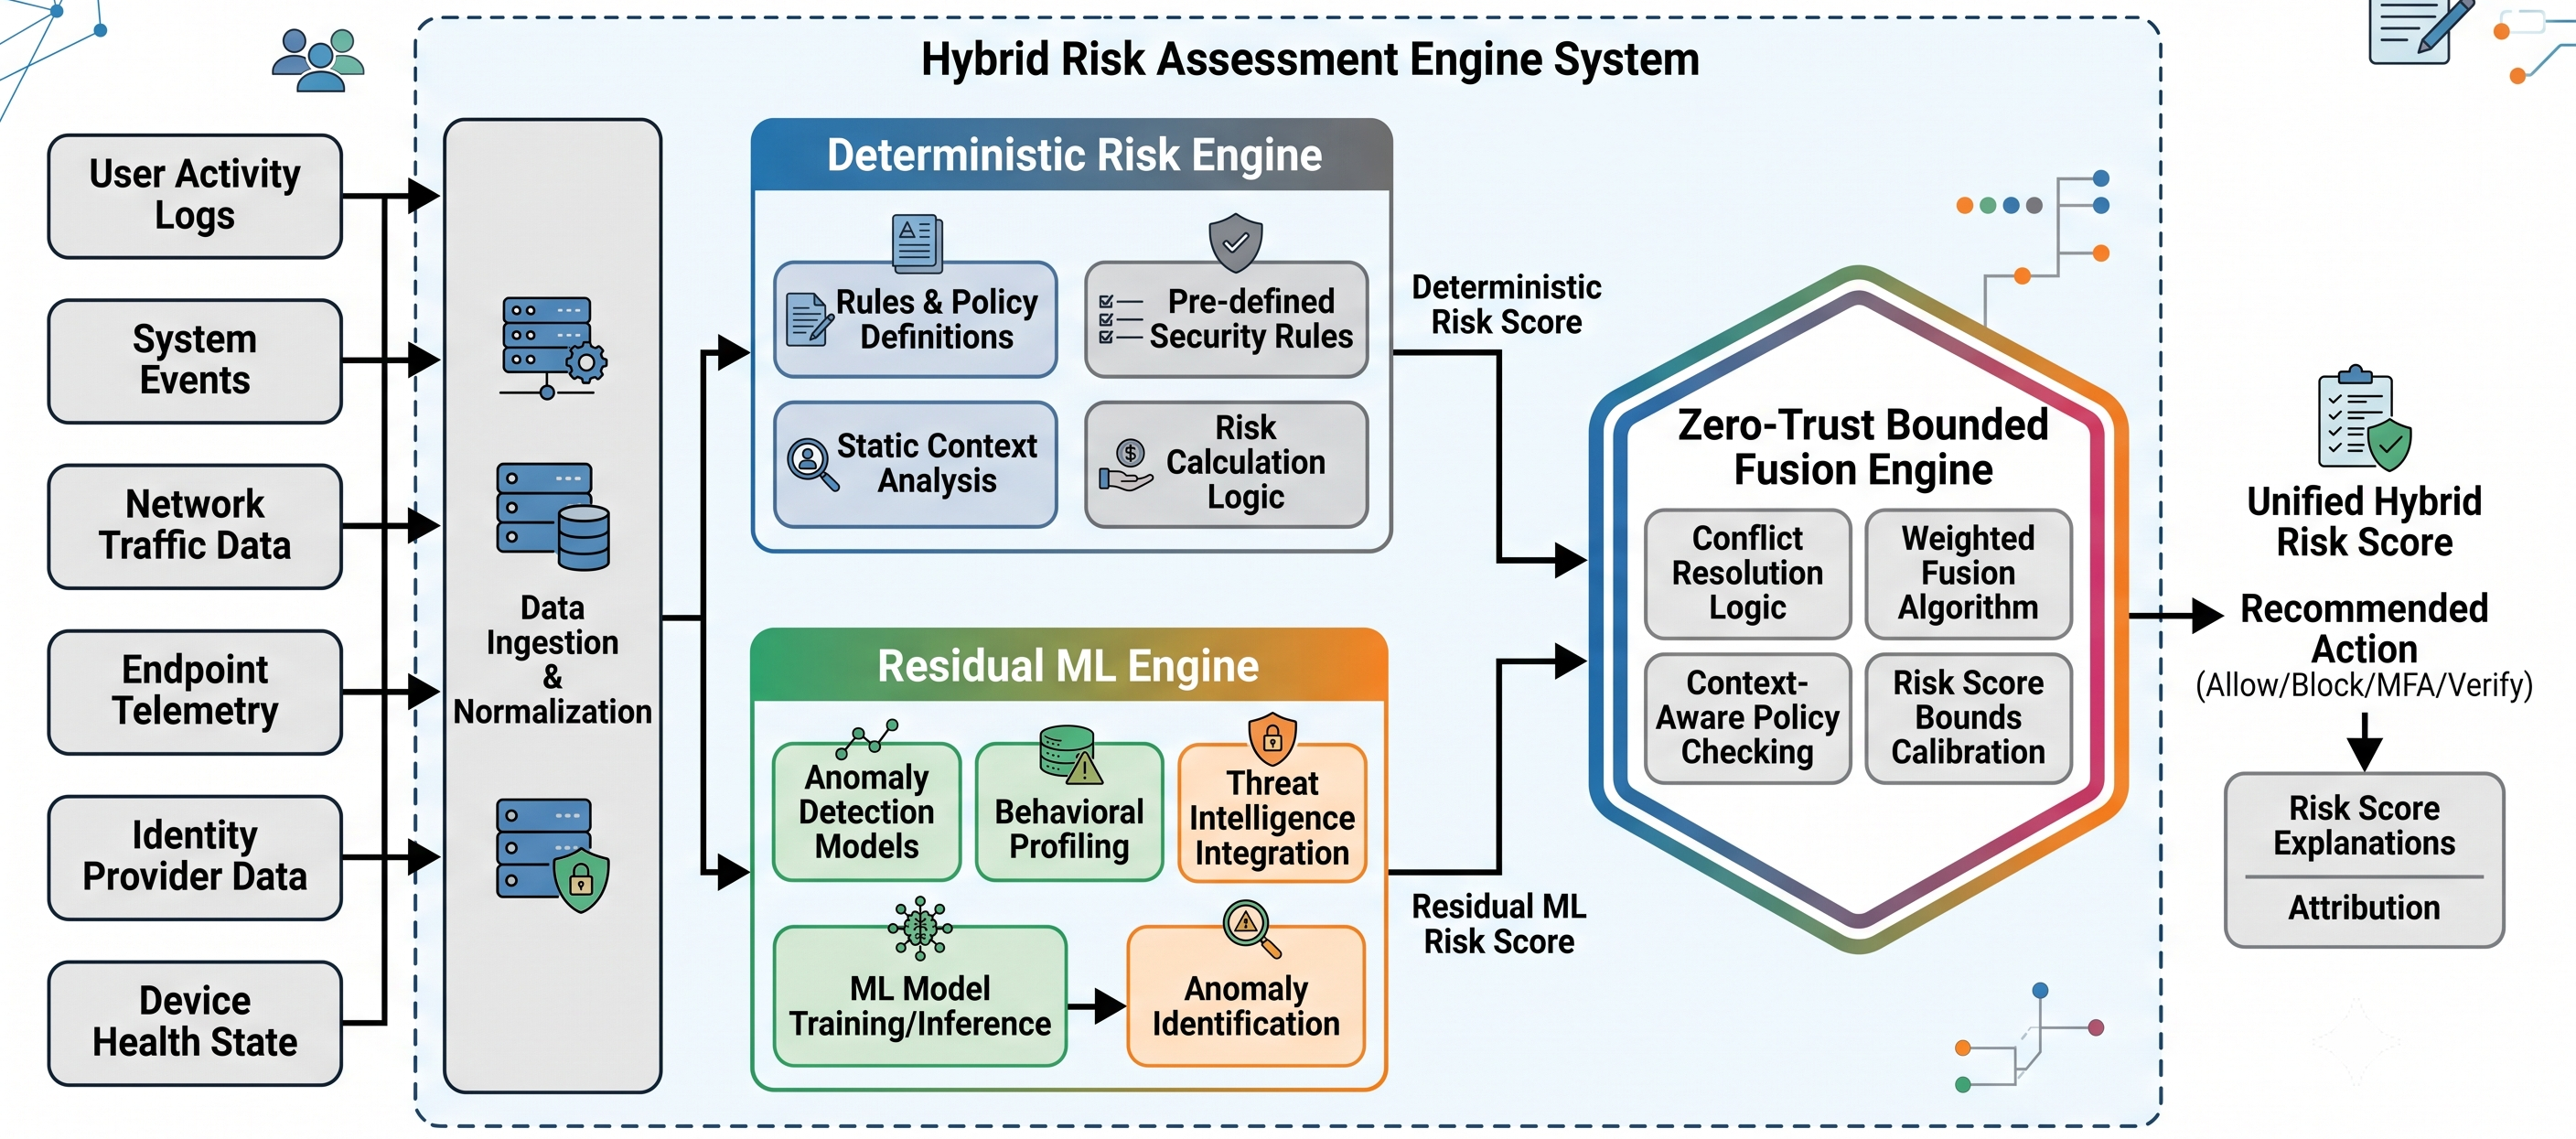
\includegraphics[width=0.90\textwidth,height=0.55\textheight,keepaspectratio]{fig6.png}
    \caption{Architectural integration across asynchronous reconnaissance modules, Verification Matrix, and Quantitative Scoring Engines.}
  \end{figure}
\end{frame}

% =====================================================================
\section{Quantitative Exposure Scoring (PDSS)}
% =====================================================================

\begin{frame}{Quantitative Vulnerability Scoring: The PDSS Formula}
  \small
  To replace informal vulnerability ratings, we define a two-track Personal Data Sensitivity Score (PDSS) mathematically bounded within a strict $0.0$ to $10.0$ interval.
  
  \vspace{0.15cm}
  \begin{block}{\centering \textbf{Deterministic Vulnerability Formulation}}
    \scriptsize
    Synthesizes core component dimensions—Sensitivity ($S$), Discoverability ($D$), Linkability ($L$), and Impact ($I$)—weighted by statistical observations and confidence:
    $$\text{Base Score} = 10.0 \times \left(0.25\,S + 0.20\,D + 0.20\,L + 0.35\,I\right)$$
    $$\text{Final Exposure} = \text{Base Score} \times \left(0.55 + 0.45 \times \text{Confidence}\right)$$
  \end{block}

  \vspace{0.15cm}
  \begin{itemize}\setlength{\itemsep}{0.15cm}
    \item \textbf{Scientific Justification of Coefficients:} Calibrated following CVSS v3.1 impact-dominance principles \footcite{cvss2019}. \textbf{Impact ($\mathbf{0.35}$)} receives the highest weight because exploited breaches cause irreversible loss, whereas \textbf{Sensitivity ($\mathbf{0.25}$)}, \textbf{Discoverability ($\mathbf{0.20}$)}, and \textbf{Linkability ($\mathbf{0.20}$)} represent preconditions that only compound severity upon exploitation.
    \item \textbf{Confirmed vs. Possible Tracks:} Explicitly isolates confirmed identities from ambiguous username candidates to prevent score inflation.
  \end{itemize}
\end{frame}

% =====================================================================
\section{Residual ML Risk Calibration}
% =====================================================================

\begin{frame}{Auxiliary Residual Risk Calibration}
  \small
  While deterministic equations provide repeatable accountability, they treat exposure events as independent. To evaluate non-linear multi-platform targeting, we integrate an Auxiliary Machine Learning Regressor.
  
  \vspace{0.20cm}
  \begin{itemize}\setlength{\itemsep}{0.22cm}
    \item \textbf{Algorithmic Selection \& Baselines:} We selected Histogram-based Gradient Boosting (\texttt{HistGradientBoostingRegressor}) over Random Forest due to its native handling of unscaled tabular security metrics, lower RAM footprint, and rapid execution speed \footcite{pedregosa2011, ke2017}.
    \item \textbf{Bounded Residual Calibration:} Rather than replacing deterministic logic, the ML engine predicts an adjustment delta ($\Delta_{\text{target}}$) clamped within a strict mathematical tolerance band ($\pm \delta_{\text{max}}$):
      $$\text{Hybrid Score} = \text{Deterministic Score} \pm \min(|\Delta_{\text{target}}|, \; \delta_{\text{max}})$$
    \item \textbf{Model Integrity Verification:} Prior to RAM loading, an integrity auditor verifies runtime SHA-256 binary digests against an immutable registry to prevent model tampering and deserialization injection exploits.
  \end{itemize}
\end{frame}

\begin{frame}{ML Experimental Evaluation \& Dataset Validation}
  \footnotesize
  \begin{columns}[T]
    \begin{column}{0.51\textwidth}
      \textbf{Model Evaluation \& Training Rigor:}
      \begin{itemize}\setlength{\itemsep}{0.12cm}
        \item \textbf{Synthetic Dataset Validation ($\mathbf{N=1,000}$):} Due to statutory privacy frameworks (GDPR, DPDP Act), harvesting real individual exposures is legally prohibitive. Synthetic profiles were mathematically formulated to preserve authentic covariance and threat distributions.
        \item \textbf{Training Protocols:} 80/20 train-test split with 5-fold cross-validation.
        \item \textbf{Empirical Convergence:} Achieved \textbf{MAE = 1.1478} and \textbf{RMSE = 1.4336}.
        \item \textbf{Sub-Group Stability:}
          \begin{itemize}\setlength{\itemsep}{0.06cm}
            \item \scriptsize Low-Risk Profiles ($n=350$): MAE $= 1.1233$
            \item \scriptsize High-Risk Profiles ($n=323$): MAE $= 1.1210$
            \item \scriptsize Medium-Risk Profiles ($n=327$): MAE $= 1.2006$
          \end{itemize}
      \end{itemize}
    \end{column}
    \begin{column}{0.49\textwidth}
      \begin{block}{\centering \textbf{Feature Importance Ranking}\\ (Correlation to Adjustment Delta)}
        \scriptsize
        \begin{enumerate}\setlength{\itemsep}{0.12cm}
          \item \textbf{Confirmed Track PDSS Score:} $0.756$
          \item \textbf{Confirmed Finding Count:} $0.672$
          \item \textbf{Maximum Base Severity Indicator:} $0.658$
          \item \textbf{Identity Leak Total Count:} $0.557$
          \item \textbf{Credential Breach Count:} $0.510$
          \item \textbf{Cumulative Severity Sum:} $0.391$
        \end{enumerate}
      \end{block}
      \vspace{0.10cm}
      \scriptsize \textit{Note: The dominance of Confirmed Track PDSS proves the ML correctly builds upon deterministic foundations.}
    \end{column}
  \end{columns}
\end{frame}

\begin{frame}{Strategic Remediation: Directed Acyclic Graph (DAG)}
  \footnotesize
  \begin{columns}[T]
    \begin{column}{0.49\textwidth}
      \textbf{Dependency-Ordered Mitigation:}
      \begin{itemize}\setlength{\itemsep}{0.15cm}
        \item Traditional security audits overwhelm users with unstructured, chaotic advice lists.
        \item Our engine models mitigation playbooks as a Directed Acyclic Graph ($G = (V, E)$) to enforce logical prerequisite ordering.
        \item \textbf{Cycle Prevention \& Complexity:} Prerequisite relationships are strictly acyclic by design. Topological ordering via Kahn's algorithm executes in $\mathcal{O}(|V| + |E|)$ worst-case linear time.
        \item \textbf{Prerequisite Example:} Enforces that a user must revoke a compromised password before attempting to configure Multi-Factor Authentication (MFA).
        \item \textbf{Urgency ROI Ranking:} Tasks are sorted by computing Return-on-Investment based on effort friction versus exposure reduction.
      \end{itemize}
    \end{column}
    \begin{column}{0.51\textwidth}
      \begin{figure}
        \centering
        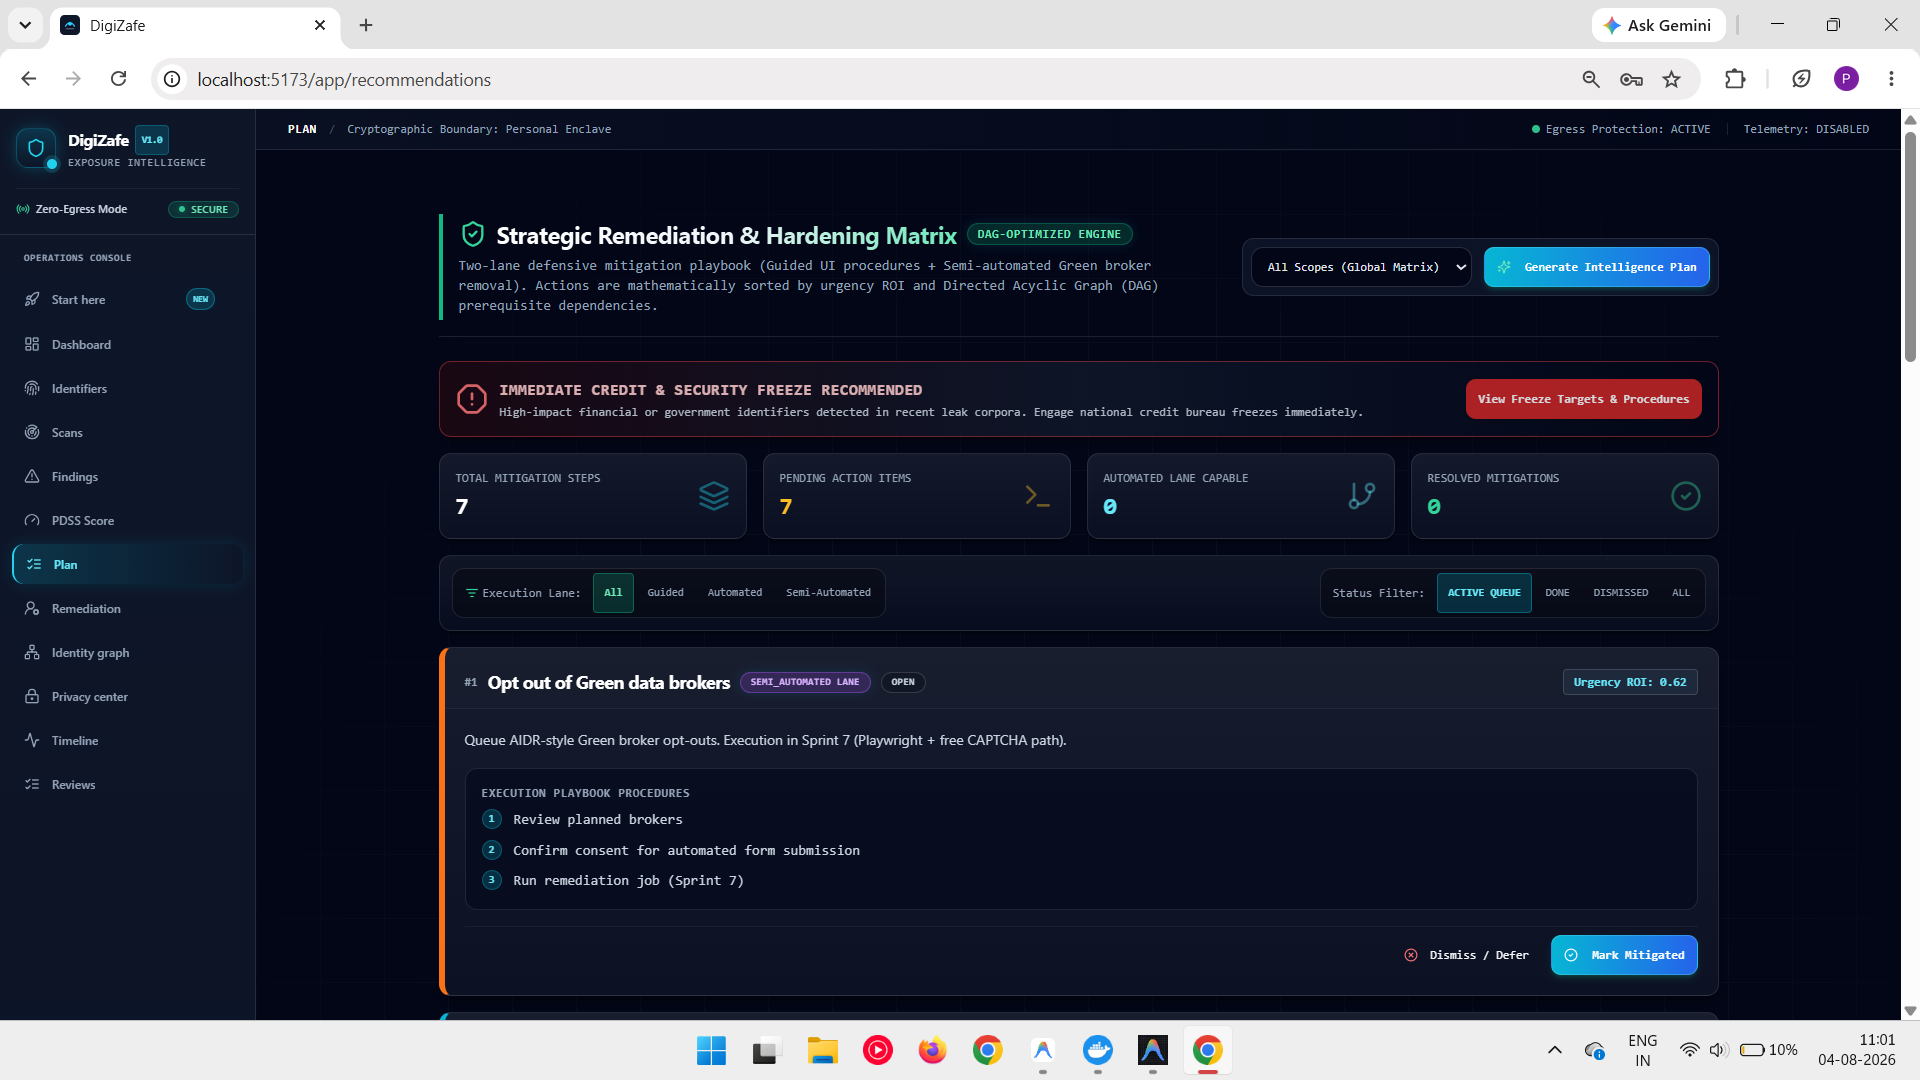
\includegraphics[width=\textwidth,height=0.55\textheight,keepaspectratio]{fig4.png}
        \caption{Strategic Remediation Matrix showcasing dependency-ordered DAG playbooks.}
      \end{figure}
    \end{column}
  \end{columns}
\end{frame}

% =====================================================================
\section{Experimental Setup \& Benchmarks}
% =====================================================================

\begin{frame}{Experimental Setup \& Implementation Stack}
  \begin{table}
    \centering
    \footnotesize
    \begin{tabular}{>{\raggedright\arraybackslash}p{4.2cm} >{\raggedright\arraybackslash}p{7.8cm}}
      \toprule
      \textbf{Architectural Layer} & \textbf{Specification / Technology Employed} \\
      \midrule
      \textbf{Presentation Tier} & React 18 Single Page Application with TypeScript \& Tailwind CSS \\
      \textbf{Client State Governance} & Zustand memory-only authentication state (Stateless Client) \\
      \textbf{Orchestration Server} & Asynchronous Python 3.12 ASGI REST API on FastAPI \footcite{fastapi2025} \\
      \textbf{Relational Persistence} & PostgreSQL 16 enforcing tenant Row-Level Security (RLS) \\
      \textbf{In-Memory Cache \& Queues} & Redis 7 buffering rate limits ($3600\text{s}$ TTL) and asynchronous tasks \\
      \textbf{OSINT Discovery Suite} & Modular Subprocess Sandbox (Maigret, Osintgram, Sherlock) \\
      \textbf{Cryptographic Primitives} & RFC 9106 Argon2id Cyphers \& HMAC-SHA256 Blind Indexing \\
      \textbf{Machine Learning Framework} & Scikit-Learn \texttt{HistGradientBoosting} with SHA-256 Registry \\
      \bottomrule
    \end{tabular}
    \caption{Experimental system stack and software framework configuration across all operational tiers.}
  \end{table}
\end{frame}

\begin{frame}{Empirical Algorithmic Benchmarks vs. Industry Baselines}
  \small
  To demonstrate real-world operational viability, we measured execution latencies directly against production containers and compared them against industry standards:
  
  \vspace{0.15cm}
  \begin{table}
    \centering
    \scriptsize
    \begin{tabular}{l r >{\raggedright\arraybackslash}p{5.8cm}}
      \toprule
      \textbf{Evaluation Metric / Engine} & \textbf{Empirical Result} & \textbf{Baseline Comparison \& Scientific Implication} \\
      \midrule
      \textbf{Automated Test Conformance} & \textbf{101 / 101 Passed} & Verified across 100\% of unit and integration test suites \\
      \textbf{Tenant Security Audit} & \textbf{0 Defects} & Guaranteed tenant data isolation via Row-Level Security \\
      \textbf{PDSS Exposure Evaluation} & \textbf{5.78 ms} & \textbf{vs. $\mathbf{\sim 150\,\text{ms}}$ Cloud REST API Baseline:} $\mathbf{25\times}$ speedup by running deterministic evaluation locally in RAM over 50 findings \\
      \textbf{DAG Playbook Generation} & \textbf{47.50 $\boldsymbol{\mu}$s} & \textbf{vs. $\mathbf{\sim 5\,\text{ms}}$ Naive Graph Sorting:} Microsecond execution via linear-time $\mathcal{O}(|V|+|E|)$ topological sorting \\
      \textbf{Identifier Canonicalization} & \textbf{20.31 $\boldsymbol{\mu}$s} & Real-time regular expression string normalization and display redaction \\
      \textbf{Argon2id Hash Derivation} & \textbf{92.34 ms} & \textbf{vs. NIST $\mathbf{>50\,\text{ms}}$ Security Target:} Calibrated to halt GPU cracking while keeping interactive login delay below perceptible thresholds \footcite{RFC9106_Argon2} \\
      \textbf{Argon2id Hash Verification} & \textbf{75.72 ms} & Seamless authentication verification without UI blocking delays \\
      \bottomrule
    \end{tabular}
  \end{table}
\end{frame}

% =====================================================================
\section{System Visual Verification}
% =====================================================================

\begin{frame}{Visual Verification 1: Onboarding \& Privacy Isolation Architecture}
  \begin{figure}
    \centering
    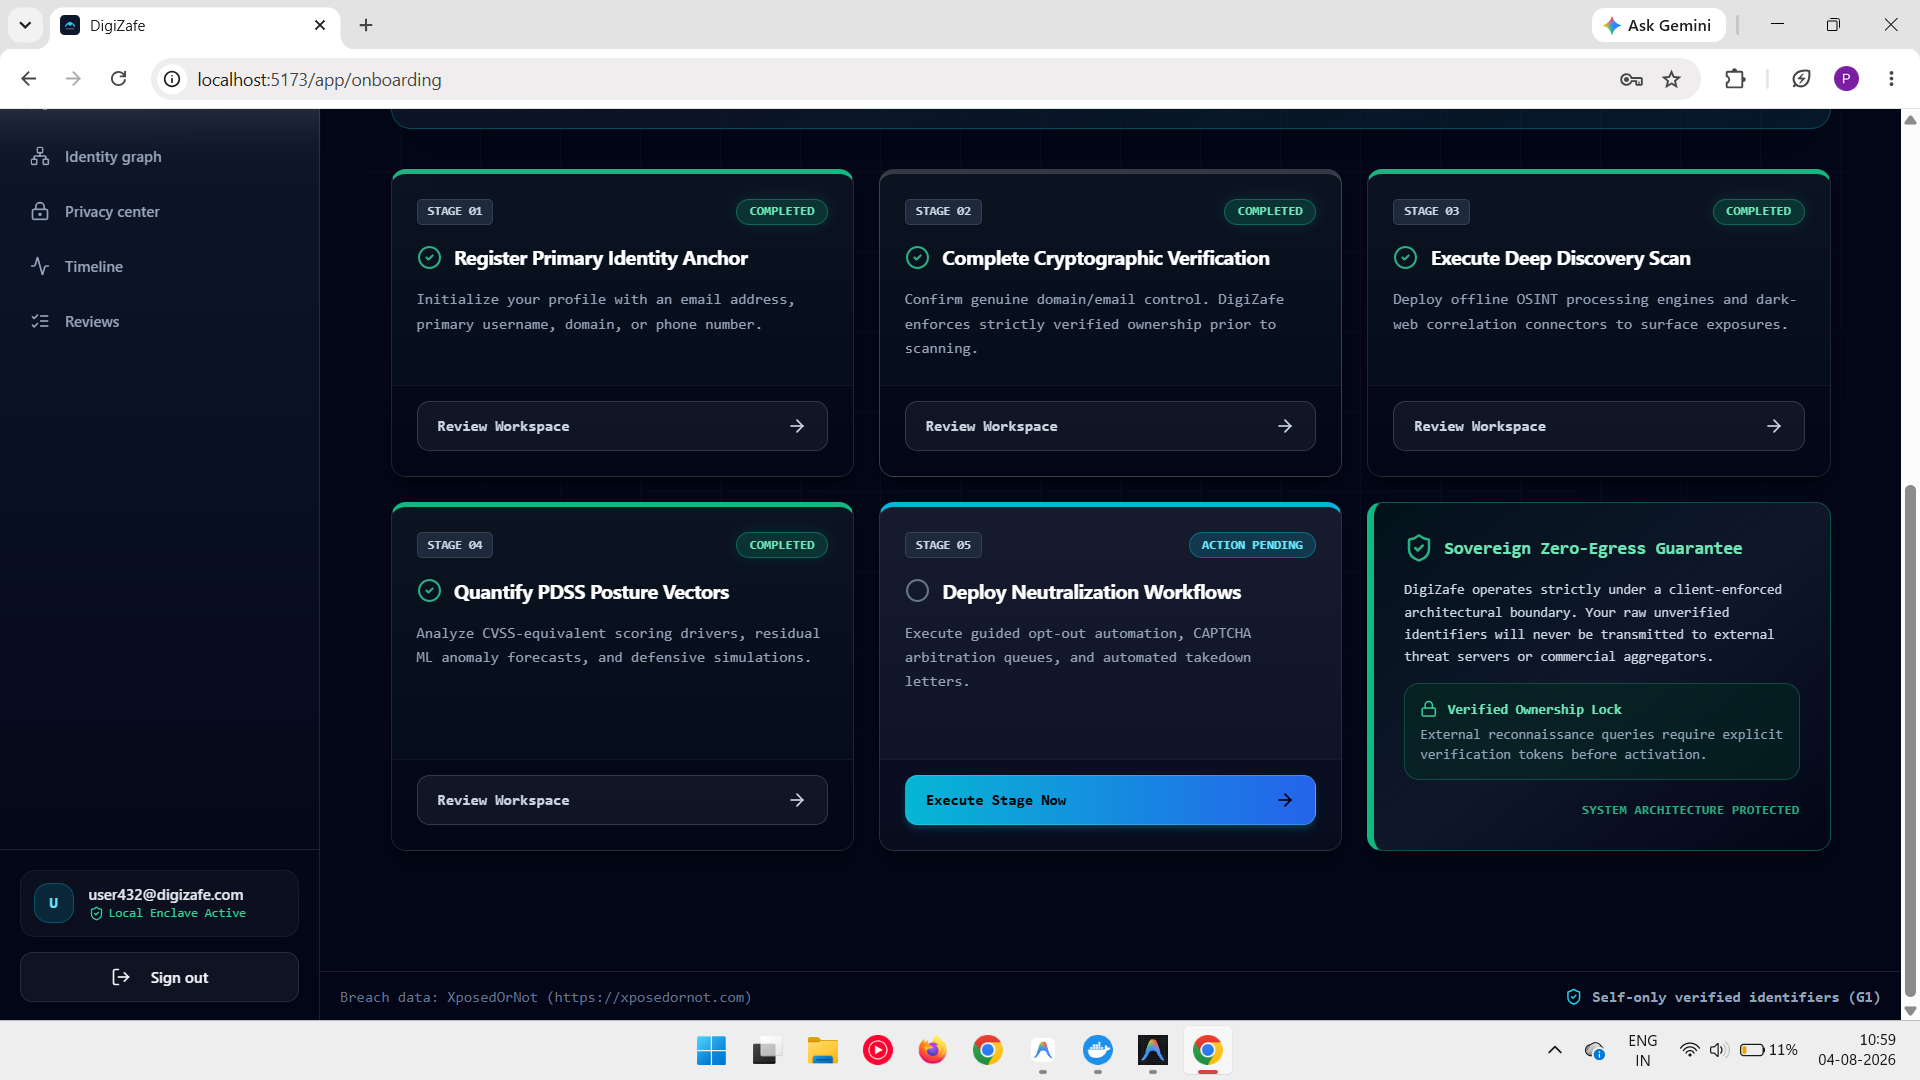
\includegraphics[width=0.88\textwidth,height=0.55\textheight,keepaspectratio]{fig1.png}
    \caption{Interactive onboarding interface establishing verified ownership and localized data encryption boundaries.}
  \end{figure}
\end{frame}

\begin{frame}{Visual Verification 2: PDSS Dashboard \& Identity Graph}
  \begin{figure}
    \centering
    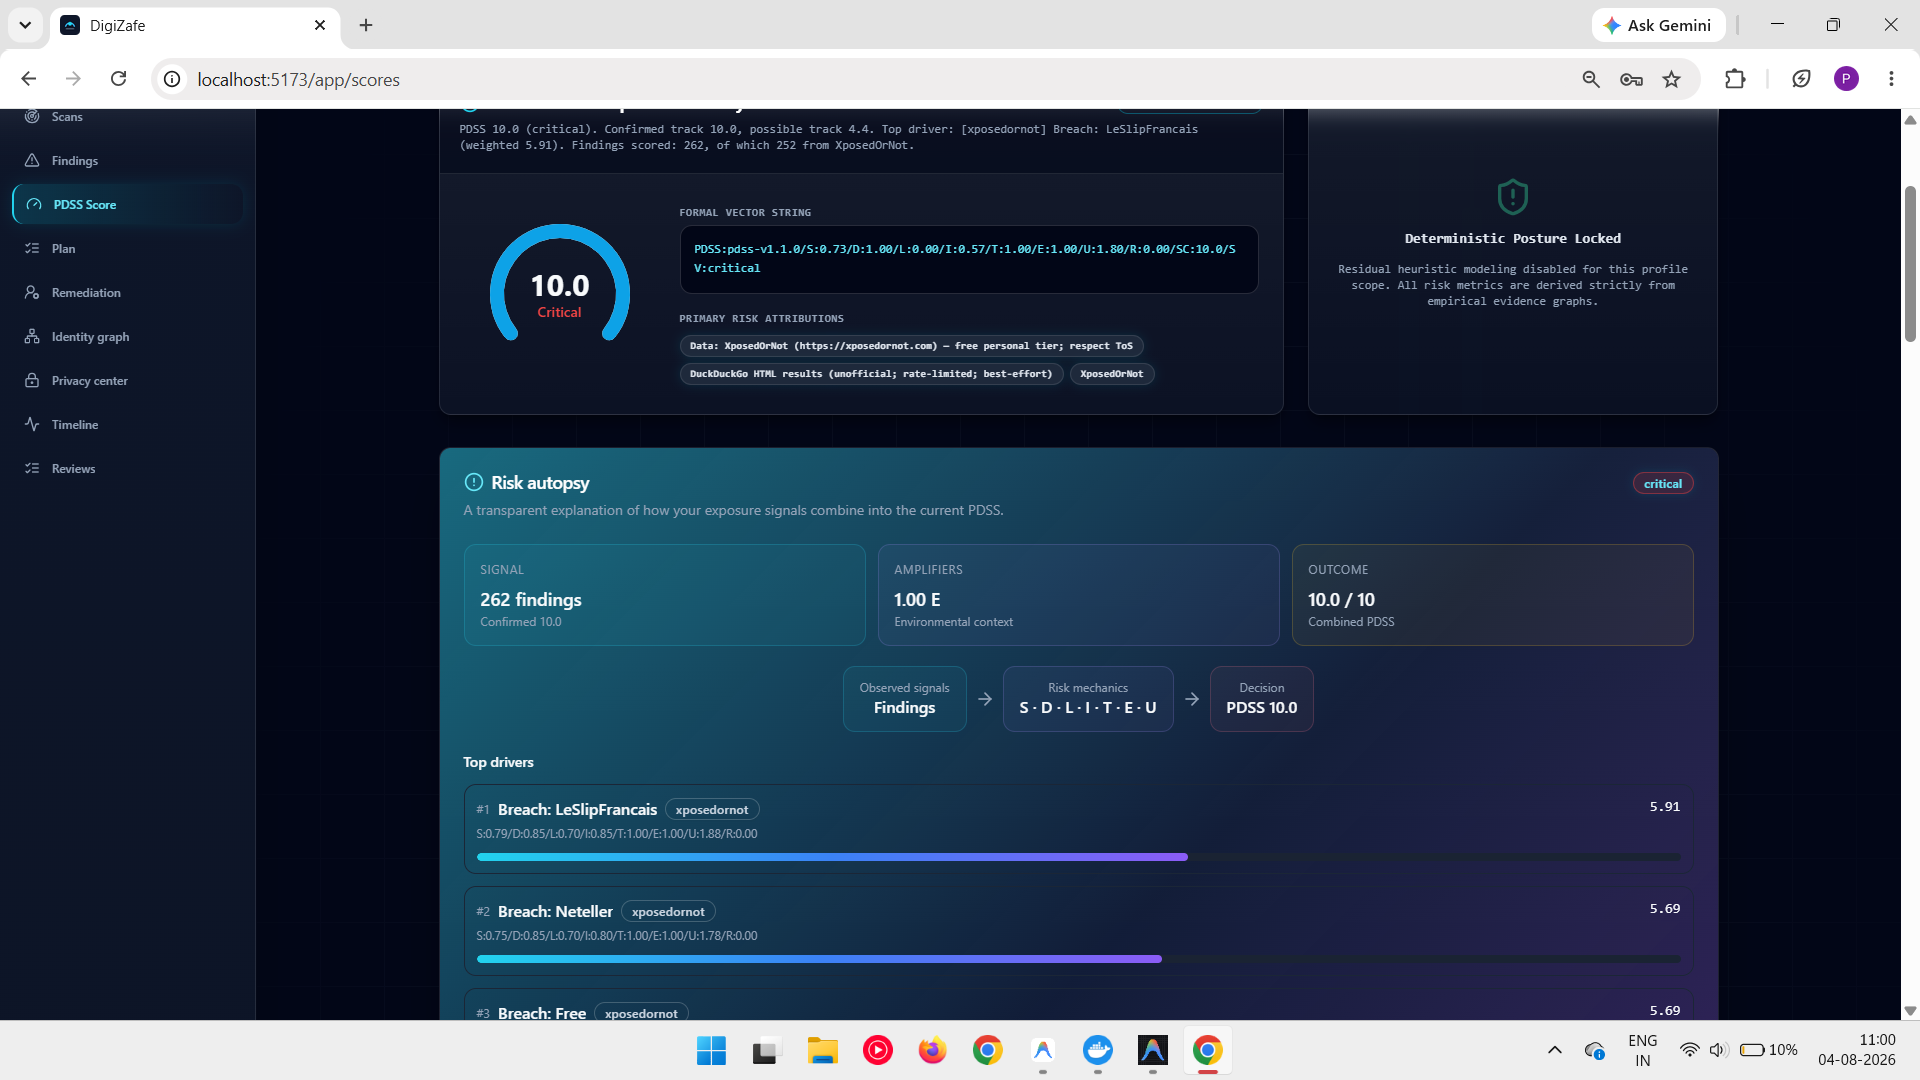
\includegraphics[width=0.88\textwidth,height=0.55\textheight,keepaspectratio]{fig2.png}
    \caption{Real-time exposure dashboard showcasing severity ratings, quantitative vectors, and force-directed linkages.}
  \end{figure}
\end{frame}

\begin{frame}{Visual Verification 3: Automated Neutralization Interface}
  \begin{figure}
    \centering
    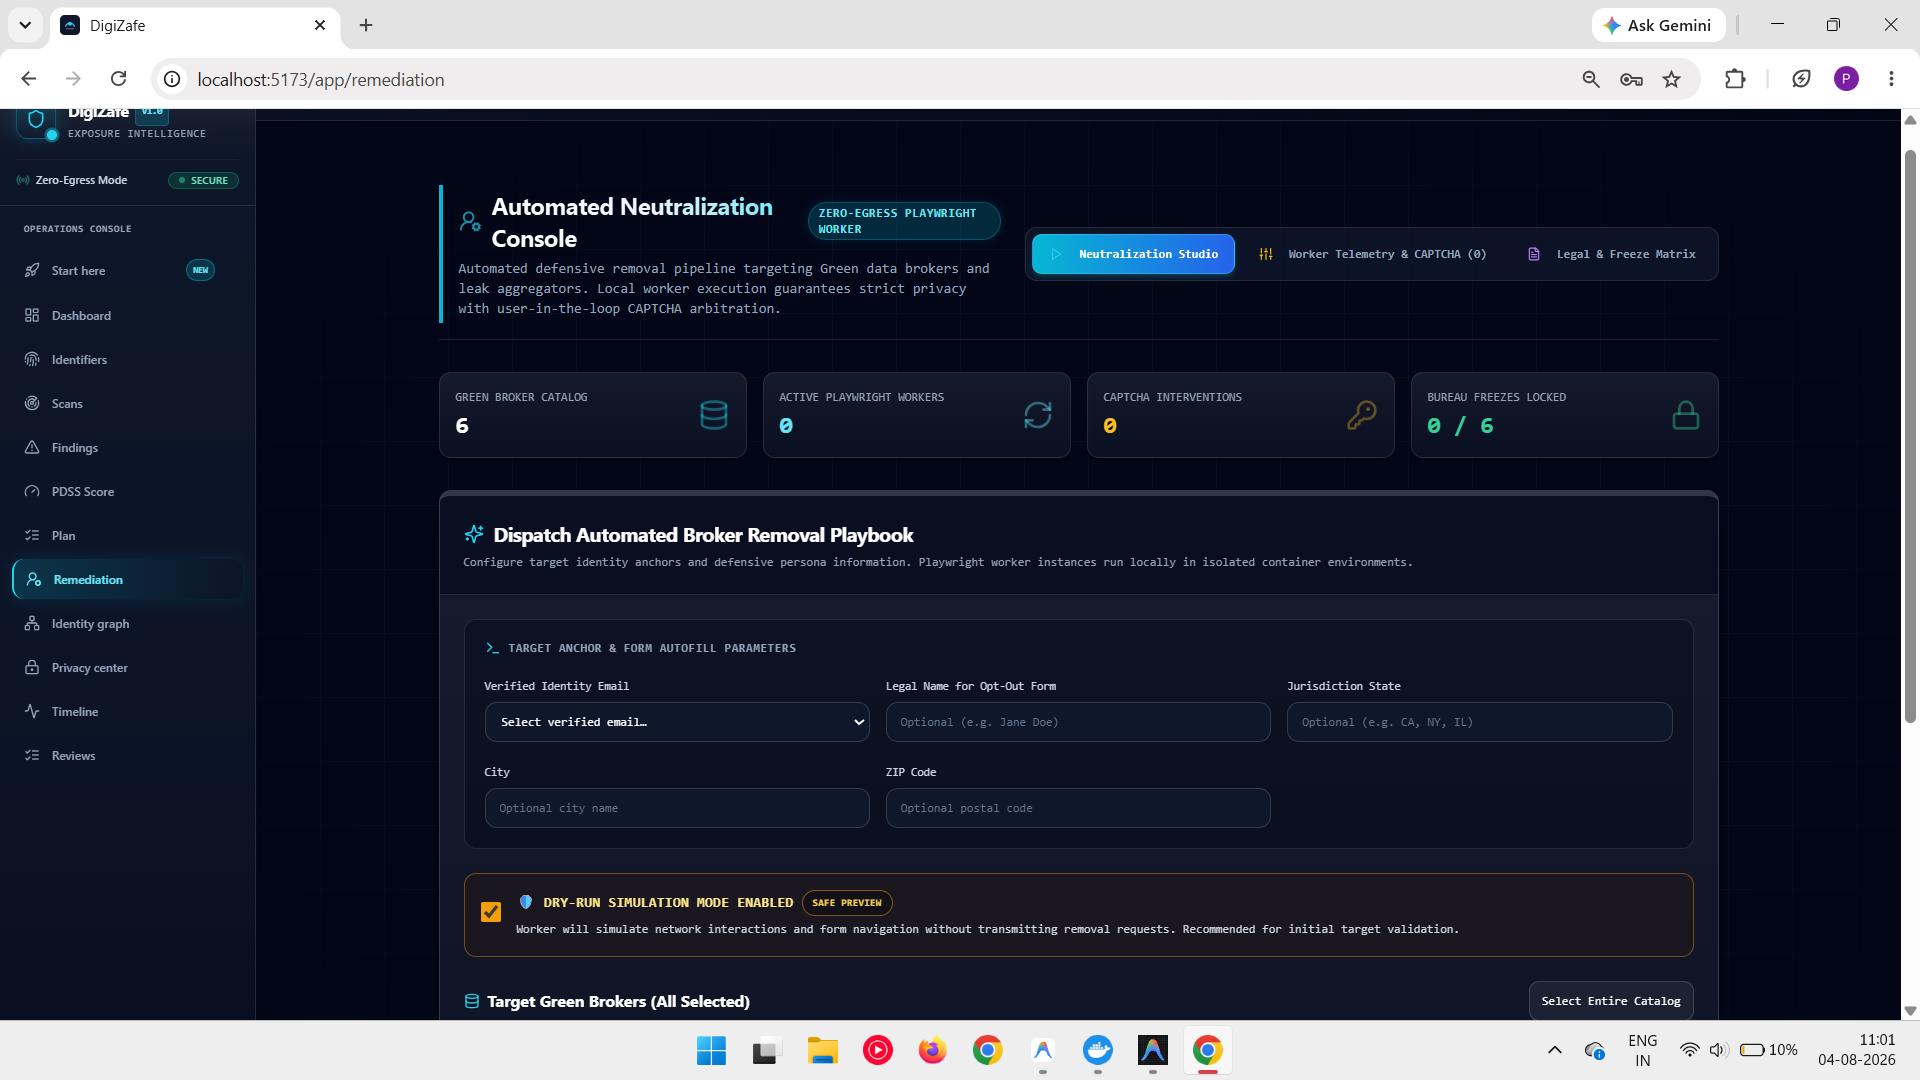
\includegraphics[width=0.88\textwidth,height=0.55\textheight,keepaspectratio]{fig5.png}
    \caption{Automated remediation dashboard managing browser takedown workers and safe dry-run simulation previews.}
  \end{figure}
\end{frame}

% =====================================================================
\section{Limitations, Future Work \& Conclusion}
% =====================================================================

\begin{frame}{Scientific Limitations \& Scope Constraints}
  \normalsize
  To maintain academic rigor, we identify three primary boundaries of the current platform implementation:
  
  \vspace{0.25cm}
  \begin{itemize}\setlength{\itemsep}{0.40cm}
    \item \textbf{Synthetic Data Reliance in Auxiliary ML:} Because real personal exposure telemetry is restricted by privacy law, the auxiliary regression model is calibrated on synthetic distribution representations ($N=1,000$) rather than longitudinal field data.
    \item \textbf{Dependency on Third-Party Target Upkeep:} Surface reconnaissance modules (Maigret, WHOIS scrapers) depend on external web structures and remain sensitive to unexpected DOM mutations or strict HTTP 429 rate-limiting blocks.
    \item \textbf{Static Dimension Weights in PDSS:} Deterministic scoring coefficients currently employ fixed heuristics adapted from CVSS v3.1 rather than dynamically optimized user domain parameters.
  \end{itemize}
\end{frame}

\begin{frame}{Engineering Solutions \& Future Work}
  \small
  \begin{itemize}\setlength{\itemsep}{0.28cm}
    \item \textbf{Conquered Engineering Challenges:}
      \begin{itemize}\setlength{\itemsep}{0.10cm}
        \item \scriptsize \textit{Rate Limiting Mitigation:} Built an in-memory Redis caching gateway ($3600\text{s}$ TTL) to absorb duplicate discovery requests and schedule compliant discovery delays.
        \item \scriptsize \textit{Model Tamper Prevention:} Deployed runtime SHA-256 hashing to verify machine learning models against an immutable registry before execution in RAM.
      \end{itemize}
    \item \textbf{Future Roadmap:}
      \begin{itemize}\setlength{\itemsep}{0.10cm}
        \item \scriptsize \textbf{Continuous Monitoring Daemons:} Integrate Celery background cron workers for automated scheduled rescans and live dark-web leak notifications.
        \item \scriptsize \textbf{Standalone Manifest V3 Extension:} Port core verification algorithms into a cross-browser extension for real-time phishing and domain reputation scoring.
        \item \textbf{FIDO2 / Passkey Support:} Upgrade authentication mechanisms to support hardware security enclaves and cryptographic passkey standards.
      \end{itemize}
  \end{itemize}
\end{frame}

% =====================================================================
\section{Conclusion}
% =====================================================================

\begin{frame}{Conclusion}
  \normalsize
  \begin{itemize}\setlength{\itemsep}{0.40cm}
    \item Successfully developed a self-governed reconnaissance platform operating under strict client privacy isolation and memory-hard authentication.
    \item Formulated an explainable quantitative exposure scoring framework (PDSS) complemented by bounded residual ML calibration (MAE of $1.1478$).
    \item Demonstrated microsecond-level performance for Directed Acyclic Graph takedown routing ($47.50\,\mu\text{s}$) and a $25\times$ speedup ($5.78\,\text{ms}$) over cloud REST baselines.
    \item Verified operational reliability and security isolation with a 100\% automated testing pass rate ($101/101$) and zero data leak vulnerabilities.
  \end{itemize}
\end{frame}

% =====================================================================
% CLOSING \& REFERENCES
% =====================================================================

{\setbeamercolor{normal text}{fg=mcmPrimaryFg,bg=mcmAlert!70}
\begin{frame}[plain,noframenumbering]
  \begin{center}
    \huge
    \textbf{Thank You}\\
    \vspace{0.8cm}
    \Large Open for Academic Defense \& Technical Discussion
  \end{center}
\end{frame}
}

\begin{frame}[allowframebreaks]{References}
  \tiny
  \printbibliography[heading=none]
\end{frame}

\end{document}
